\documentclass[12pt]{article}
\usepackage{xeCJK}
% 设置文档正文字体为宋体
\setCJKmainfont[BoldFont=SimHei]{SimSun}
\setCJKmonofont{SimSun}     % 设置缺省中文字体
\parindent 2em              % 段首缩进

\title{32位最大公约数处理器设计}
\author{张秉异~顾晨昊~叶汉辰}
\date{\today}

\usepackage{amsmath}
\usepackage{amssymb}
\usepackage{amsfonts}
\usepackage{graphicx}

\usepackage{geometry}
\usepackage{fancyhdr}
\usepackage{listings}
\usepackage{fontspec}
\usepackage[colorlinks,linkcolor=blue]{hyperref}

\usepackage{cases}
\usepackage{latexsym}
\usepackage{fvrb-ex}
\usepackage{etex}
%\usepackage{caption,subcaption}

\usepackage{multirow}
\usepackage{algorithm}  
\usepackage{algorithmicx}  
\usepackage{algpseudocode}
\usepackage{float}  
\usepackage{dirtree}  
\renewcommand{\algorithmicrequire}{\textbf{Input:}}
\renewcommand{\algorithmicensure}{\textbf{Output:}}
\newcommand{\HRule}{\rule{\linewidth}{0.5mm}}

\newfontfamily\Consolas{Consolas}
\lstset{
language=Verilog,
numbers=left,
breaklines=true,
tabsize=2,
frame=single,
basicstyle=\Consolas\small}

\geometry{a4paper}
\geometry{
left=3cm,
right=3cm,
top=3cm,
bottom=3cm,}
  
\pagestyle{fancy}
\lhead{张秉异~顾晨昊~叶汉辰}
\chead{}
\rhead{32位最大公约数处理器设计}
\lfoot{}
\cfoot{\thepage}
\rfoot{}
\renewcommand{\headrulewidth}{0.4pt}
\renewcommand{\headwidth}{\textwidth}
\renewcommand{\footrulewidth}{0pt}
\setlength{\parindent}{2.45em}

\begin{document}
\begin{titlepage} 
\begin{center}
\includegraphics[width=0.4\textwidth]{./fdulogo}\\[2cm] 
\textsc{\huge 数字信号处理的VLSI设计}\\[0.8cm]
\textsc{\huge 32位最大公约数处理器设计}\\[3cm] 
\large 17212020116~张秉异 \\17212020116~顾晨昊 \\17212020116~叶汉辰
\vfill {\large \today} 
\end{center} 
\end{titlepage}

\tableofcontents
\newpage

\section{设计指标}
\subsection{设计目标}
设计一个计算两个32位整数最大公约数(GCD)的处理器。

\subsection{输入}
\begin{itemize}
\item OPA:~32-bit,~操作数一;
\item OPB:~32-bit,~操作数二;
\item START:启动信号;
\item RESET:复位信号;
\item CLK:系统时钟。
\end{itemize}

\subsection{输出}
\begin{itemize}
\item DONE:指示输出。
\item RESULT:32-bit,最大公约数(GCD);
\end{itemize}

\subsection{要求}
\begin{itemize}
\item 采用二元的最大公约数算法,即欧几里德算法(Eucldean GCD Algorithm);
\item 基于功耗优先(Power-Efficient)与性能优先(performance-Efficient)的原则,设计两种不同的VLSI实现方案;其中,一种方案使用Altera公司的FPGA设计流程实现,另一种方案使用标准的ASIC实现流程
\end{itemize}


\subsection{总模块框图}
整个系统的模块框图如下所示:
\begin{figure}[H]
\begin{center}
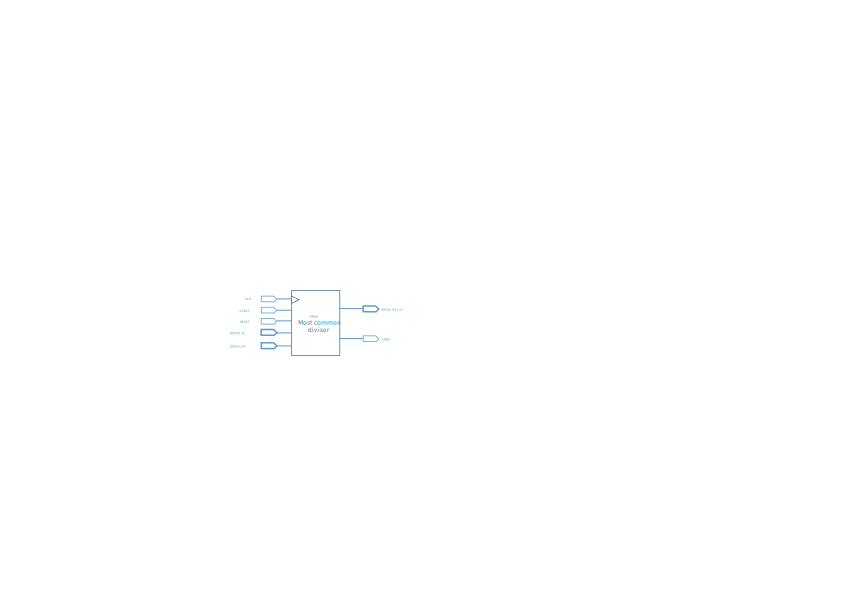
\includegraphics[width=0.8\textwidth]{./workflow/32bit_most_common_divisor.jpg}
\caption{总模块框图}
\end{center}
\end{figure}
%%%%%%%%%%%%%%%%%%%%%%%%%%%%%%%%%%%%%%%%%%%%%%%%%%%%%%%%%%%%%%%%%
%%%                                                           %%%
%%%                                                           %%%
%%%                                                           %%%
%%%%%%%%%%%%%%%%%%%%%%%%%%%%%%%%%%%%%%%%%%%%%%%%%%%%%%%%%%%%%%%%%
\section{算法}

\subsection{欧几里得算法}
\subsubsection{算法概述}
欧几里得算法又称\textbf{辗转相除法},用于计算两个整数a,b的最大公约数。其计算原理依赖于下面的定理:gcd函数就是用来求(a,b)得最大公约数的。gcd函数的基本性质:
\begin{equation}
gcd(a,b) = gcd(b,a) = gcd(-a,b) = gcd(|a|,|b|) \label{oringal_gcd}
\end{equation}


\subsubsection{公式表述}
$$gcd(a,b) = gcd(b,a~mod~b)$$
证明: a可以表示成为$a = kb+r$, 则$r = a~mod~b$

假设d是a,b的一个公约数,则有

$d|a$, $d|b$,而$r = a-kb$,因此$d|r$

因此d是$(b,a~mod~b)$的公约数

假设d是$(b,a~mod~b)$的公约数,则

$d|b$, $d|r$, 但是$a = kb+r$

因此d也是$(a,b)$的公约数

因此$(a,b)$和$(b,a~mod~b)$的公约数是一样的,其最大公约数也必然相等,得证。

\subsubsection{代码表述}
欧几里得算法用C语言代码表述如下,假设$a>b$:
\lstset{language=C}
\begin{lstlisting}
int gcd(int a, int b)
{
	if(b == 0)
		return a;
	return
		gcd(b, a%b)
}
\end{lstlisting}

\subsection{stein算法}

Stein算法是是一种计算两个数最大公约数的算法,是针对欧几里德的算法,是针对欧几里德算法在对大整数进行运算时,需要试商导致增加运算时间的缺陷而提出的改进算法。

欧几里德算法是计算两个数最大公约数的传统算法,无论从理论还是从实际效率上都是很好的。但是却有一个致命的缺陷,这个缺陷在素数比较小的时候一般是感觉不到的,只有在大素数时才会显现出来。

一般实际应用中的整数很少会超过64位(当然现在已经允许128位了),对于这样的整数,计算两个数之间的模是很简单的。对于字长为32位的平台,计算两个不超过32位的整数的模,只需要一个指令周期,而计算64位以下的整数模,也不过几个周期而已。但是对于更大的素数,这样的计算过程就不得不由用户来设计,为了计算两个超过64位的整数的模,用户也许不得不采用类似于多位数除法手算过程中的试商法,这个过程不但复杂,而且消耗了很多CPU时间。对于现代密码算法,要求计算128位以上的素数的情况比比皆是,设计这样的程序迫切希望能够抛弃除法和取模。
\subsubsection{stein算法流程}
\begin{enumerate}
\item 如果$A_{n} = B_{n}$,~那么$A_{n}$(或$B_{n}$)*$C_{n}$是最大公约数,算法结束
\item 如果$A_{n} = 0$,~$B_{n}$是最大公约数,算法结束
\item 如果$B_{n} = 0$,~$A_{n}$是最大公约数,算法结束
\item 设置$A_{1} = A$,~$B_{1} = B$和$C_{1} = 1$
\item 如果$A_{n+1} = A_{n}/2$,~$B_{n+1} = B_{n}/2$,~$C{n+1} = C_{n}*2$(注意,乘2只要把整数左移一位即可,除2只要把整数右移一位即可)
\item 如果$A_{n}$是偶数,$B_{n}$不是偶数,则$A_{n+1} = A_{n}/2$,~$B_{n+1} = B_{n}$,~$C_{n+1} = C{n}$
\item 如果$B_{n}$是偶数,$A_{n}$不是偶数,则$B_{n+1} = B_{n}/2$,~$A_{n+1} = A_{n}$,~$C_{n+1} = C_{n}$
\item 如果$A_{n}$和$B_{n}$都不是偶数,则$A_{n+1} = |A_{n} - B_{n}|/2$,~$B_{n+1} = min(A_{n},B_{n})$,~$C_{n+1} = C_{n}$
\item $n$加1,转1
\end{enumerate}
\subsubsection{stein算法代码}
\lstset{language=C}
\begin{lstlisting}
#define CHECK(a) (!(1&(a)))
#define CLEAN2(a) while(CHECK(a))a=a>>1
#define BIGERA if(a > b)(t = a, a = b, b = t)

int gcd(int a, int b)
{
	int c_2 = 0, t;
	while ((CHECK(a)) && (CHECK(b)))
	{
		a = a >> 1;
		b = b >> 1;
		c_2++;
	}
	CLEAN2(a);
	CLEAN2(b);
	BIGERA;
	while (a = ((a - b) >> 1))
	{
		CLEAN2(a);
		BIGERA;
	}
	return b << c_2;

}
\end{lstlisting}

\subsection{改进的stein算法}

\subsubsection{gcd和stein算法分析}
\textbf{gcd算法}具有算法简单,通过简单递归就能实现的特点。但是gcd算需要递归地用到除法,32-bit的除法在硬件设计中的开销非常大。在硬件实现上具有以下缺点:

\begin{itemize}
\item 关键路径长,需要多级流水线切割
\item 面积大,在实现高性能的多级流水线比较困难
\end{itemize}

\textbf{stein算法}通过运用了最大公约数的性质,使用了简单的减法和位移的操作,在硬件实现上比较简单,而且对于32-bit的操作数,最大的操作数每次迭代都会衰减$1/2$,这样整个算法最多只需要63次就能完成迭代。所以stein算法迭代周期少,控制简单非常适合做高性能的计算。

但是对于一些特殊的情况仍然需要改善。由于算法的结束的条件是$A_{n} = B_{n}$,~$A_{n} = 0$,~$B_{n} = 0$。所以例如当$A = 100001$, $B = 1$时需要多次迭代才能完成计算。计算过程如下:

start:
\begin{enumerate}
\item $A_{0} = 100001,~B_{0} = 1$
\item $A_{1} = (A_{0} - B{0})/2 = 50000,~B_{1} = 1$
\item $A_{2} = A_{1}/2 = 25000,~B_{2} = 1$
\item $A_{2} = A_{1}/2 = 25000,~B_{2} = 1$
\item $A_{3} = A_{2}/2 = 12500,~B_{3} = 1$
\item $A_{4} = A_{3}/2 = 6250,~B_{4} = 1$
\item $A_{5} = A_{4}/2 = 6250,~B_{5} = 1$
\item $A_{6} = A_{5}/2 = 3125,~B_{6} = 1$
\item $A_{7} = (A_{6} - B_{6})/2 = 1562,~B_{7} = 1$ 
\item $A_{8} = A_{7}/2 = 781,~B_{8} = 1$ 
\item $A_{9} = (A_{8} - B_{8})/2 = 390,~B_{9} = 1$ 
\item $A_{10} = A_{9}/2 = 195,~B_{10} = 1$
\item $A_{11} = (A_{10} - B_{10})/2 = 97,~B_{11} = 1$ 
\item $A_{12} = (A_{11} - B_{11})/2 = 48,~B_{12} = 1$ 
\item $A_{13} = A_{12}/2 = 24,~B_{13} = 1$
\item $A_{14} = A_{13}/2 = 12,~B_{14} = 1$
\item $A_{15} = A_{14}/2 = 6,~B_{15} = 1$
\item $A_{16} = A_{15}/2 = 3,~B_{16} = 1$
\item $A_{17} = (A_{16} - B_{16})/2 = 1,~B_{16} = 1$ 
\end{enumerate}
end

所以计算比较直观的$A = 100001$,$B = 1$两个数的最大公约数就需要19次迭代。这样大大浪费了计算时间和计算资源,在低功耗设计中是不可取的。因为在低功耗设计中需要做尽可能少的运算。

而且为了更加精确的对比gcd算法的迭代周期和stein算法的迭代中,我们小组进行了精确的matlab仿真分析,仿真脚本和结果在\textit{ASIC-euclidean\textbackslash matlabmodel}里面。我们在$(0,2^{32}-1)$范围之内,随机生成了1000万对随机整数,分别用gcd算法和stein算算法来求解最大公约数,并且统计平均计算周期,最后结果如表\ref{average_iteration}所示。

\begin{table}[!htb]
\centering
\begin{tabular}{cc}
\hline 
gcd & stein \\
\hline 
18.2592 & 42.7365\\
\hline 
\end{tabular}
\caption{\textbf{gcd}与\textbf{stein}算法平均计算迭代次数}
\label{average_iteration}
\end{table}


其中,stein算法的平均迭代次数达到了42.7365次,远远高于欧几里得算法(gcd)算法的平均迭代次数18.2592次。经过统计直方图分析,迭代次数的分布统计如下图\ref{gcd_hist}和图\ref{stein_hist}所示:

\begin{figure}[H]
\begin{minipage}[t]{0.5\linewidth}
\centering
\includegraphics[width=3in]{./matlab/gcd_hist.eps}
\caption{gcd算法迭代次数统计直方图}
\label{gcd_hist}
\end{minipage}%
\begin{minipage}[t]{0.5\linewidth}
\centering
\includegraphics[width=3in]{./matlab/stein_hist.eps}
\caption{stein算法迭代次数统计直方图}
\label{stein_hist}
\end{minipage}
\end{figure}

对于32-bit的数,欧几里得算法的迭代次数大都分布在(12, 25)之间,算法的迭代周期大都分布在(35,50)之间。所以stein算法的平均迭代周期约为gcd算法的2倍多。


\subsubsection{改进的stein算法}
在上一小节中,我们说到了stein算法非常适合用来做硬件实现,因为stein算法只包含了简单的\textbf{奇偶判断}、\textbf{移位}、\textbf{相减}、\textbf{比较大小}等计算。相比较与原始的欧几里得算法有了较大的改善。但是我在上一节,也发现一个问题就是stein算法的迭代周期比欧几里得算法的迭代次数要长。造成这一个问题的原因经过我们分析为:

\begin{quote}
当两个操作数相差较大时,stein算法对于较大的操作数不能有效的衰减。例如,对于一组操作数(1000000001,1),在stein算法中迭代时,下一组操作数为(500000000,1),而在gcd算法中迭代时,下一组操作数位(1,1)。\textbf{所以gcd算法对于相差较大的操作数能够有效衰减,而stein只能以约为1/2的衰减速率来衰减}。
\end{quote}

因此,我们分析了stein算法不足的原因所在。所以在算法设计中,我们小组对stein算法不能有效处理两个相差较大操作数的缺陷进行改进————\textbf{当两个操作数相差较大的时候,我们增大较小操作数的数量级,使得其与较大操作数的数量级一致,然后再进入下一次迭代。},是数量级一致的操作,通过硬件中简单的操作数移位就可以实现。优化的stein算法的伪代码如算法\ref{optimized_stein_algorithm}所示:

\begin{algorithm}[H]
\caption{ Framework of optimized stein algorithm} 
\label{optimized_stein_algorithm}  
\begin{algorithmic}[1]
\Require 
	opa,opb 
\Ensure
	result
\While{$(opa \neq opb)and(opa \neq 0)and((opb \neq 0))$}
	\State $opa = max(opa,opb)$,$opb = min(opa,opb)$ ;
	\State $lengthOFopa = binaryLen(opa)$,$lengthOFopb = binaryLen(opb)$;
 	\State $lengthdiff = lengthOFopa - lengthOFopb$;
 	\State $opa = abs(opa - opb << lengthdiff)$;
\EndWhile
\If{$opa = opb$}
 \State $result = opa$
\EndIf
\If{$opa = 0$}
 \State $result = opb$
\EndIf
\If{$opb = 0$}
  \State $result = opa$
\EndIf
\end{algorithmic} 
\end{algorithm}

再对原来的stein算法优化的基础上,我们在matlab中对优化的stein进行仿真,同样的,我们随机取得1000万对随机数,得到平均迭代次数如表\ref{average_iteration_optimized_stein}所示为23.7273次。

\begin{table}[H]
\centering
\begin{tabular}{c}
\hline 
optimized stein \\
\hline 
23.5273\\
\hline 
\end{tabular}
\caption{\textbf{optimized stein}算法平均计算迭代次数}
\label{average_iteration_optimized_stein}
\end{table}

\begin{figure}[H]
\begin{center}
\includegraphics[width=0.5\textwidth]{./matlab/stein_op_hist.eps}
\caption{优化的stein算法迭代次数统计直方图}
\end{center}
\end{figure}

我们通过优化的stein算法,在原来的stein算法的基础上将迭代中期的次数从42.7365减少到了
23.7273次,与gcd算法的平均18.2592次迭代相接近。而且优化的gcd算法包含了\textbf{选择判断有效位数},\textbf{比较},\textbf{移位},\textbf{减法}操作,省去了复杂的除法操作。由于复杂的除法操作在硬件实现中不仅面积开销大,而且功耗高。所以优化的stein算法非常适合与低功耗的设计。

%%%%%%%%%%%%%%%%%%%%%%%%%%%%%%%%%%%%%%%%%%%%%%%%%%%%%%%%%%%%%%%%%
%%%                                                           %%%
%%%                                                           %%%
%%%                                                           %%%
%%%%%%%%%%%%%%%%%%%%%%%%%%%%%%%%%%%%%%%%%%%%%%%%%%%%%%%%%%%%%%%%%
\section{高性能设计}
\subsection{设计综述}
经过第二章对算法的分析,在高性能的设计中,我们采用了stein算法,根据计算stein算法最多需要63次迭代完成gcd计算。为了尽可能提高gcd处理器的数据吞吐率,我们将63次迭代展开为63级流水线,同时尽可能减小每一级流水线的计算延迟,提高运行频率。数据输入模块和数据输出模块分别构成一级流水线,故总流水线级数为65级。

在设计过程中,为了降低每一级流水线的计算延迟,我们考虑过将每一次迭代进行进一步的流水线划分,构成126或更多级流水线,但实际设计和测试后,发现该做法并不能取得很好的收益。该部分将在RTL电路设计的流水线计算模块一节详细阐述。

\subsection{RTL电路设计}
高性能设计的电路设计文件在hp/rtl/文件夹中,其中包含三个子模块和一个顶层模块gcd\_top。gcd\_input为数据输入模块,gcd\_plc为流水线计算模块,gcd\_output为数据输出模块。gcd\_top提供了设计要求中的输入和输出接口,例化了1个gcd\_input模块、63个gcd\_plc模块、1个gcd\_output模块,构成总共65级流水线,并对它们进行了顶层的连接。顶层模块的结构框图如下图所示。

\begin{figure}[H]
\begin{center}
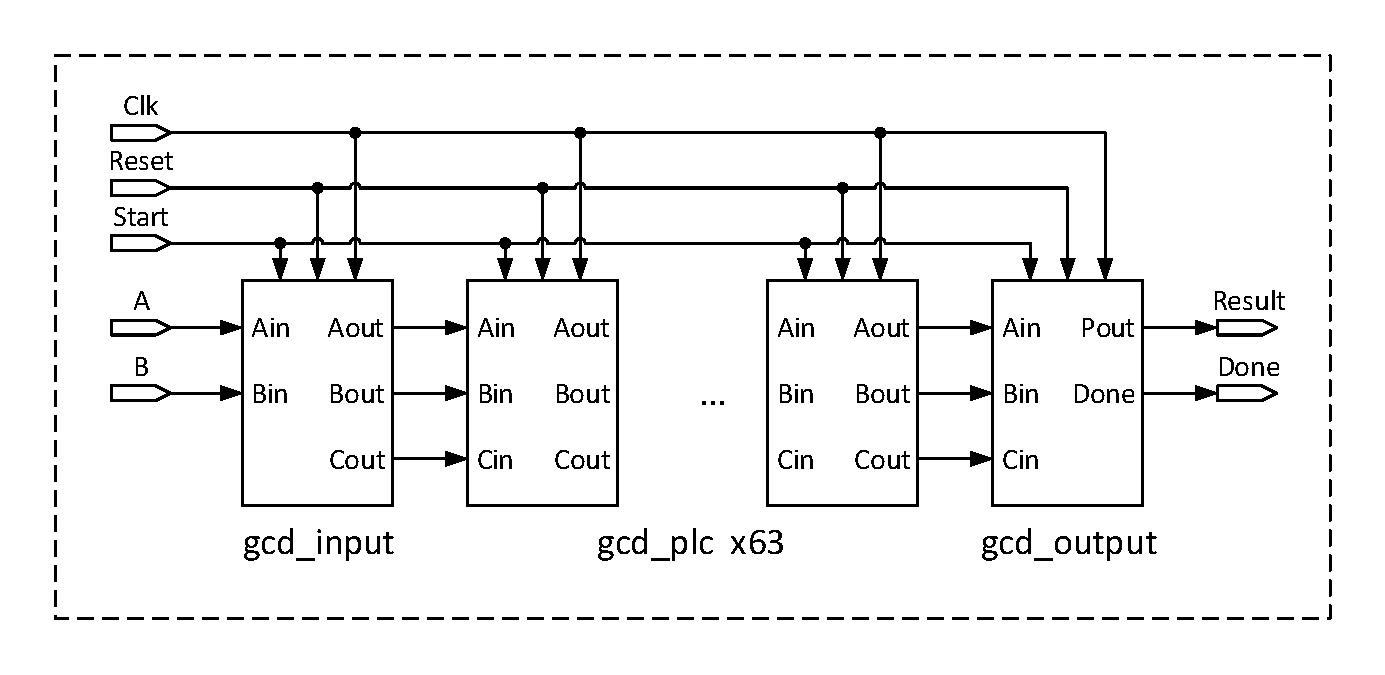
\includegraphics[width=0.9\textwidth]{./yhc_hp/gcd_top.eps}
\caption{gcd\_top模块结构框图}
\end{center}
\end{figure}

需要指出,在本设计中,Reset信号置低时,流水线中所有寄存器清零;Start信号置低时,流水线中所有寄存器的值保持不变,即进入halt状态,当Start信号重新置高时,运算继续进行;Done信号仅在有有效计算结果输出时置高。下面将分别对三个子模块设计进行详细说明。

\subsubsection{数据输入模块}
该模块将输入的A、B传送到流水线计算模块中进行计算,同时为C赋初值。该模块的电路图如下图所示。

\begin{figure}[H]
\begin{center}
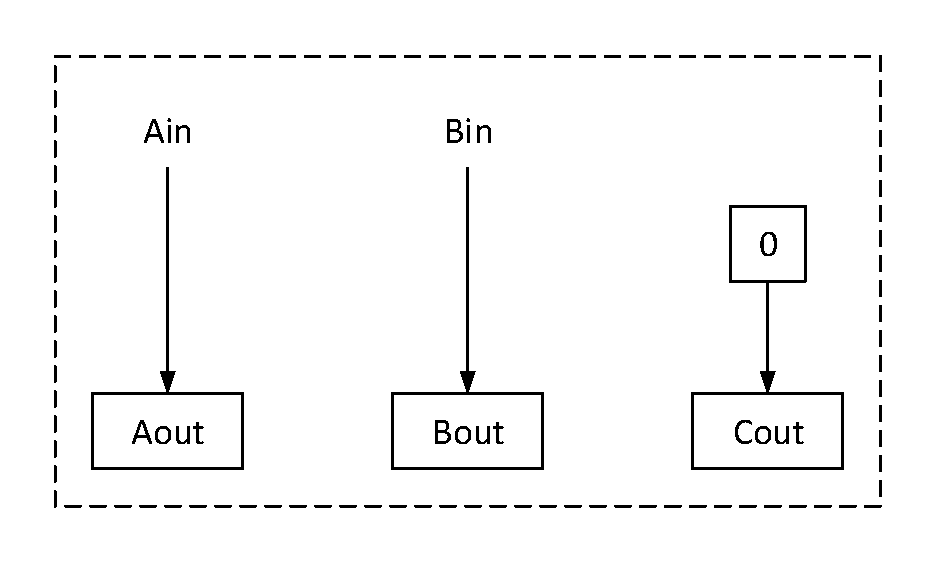
\includegraphics[width=0.6\textwidth]{./yhc_hp/gcd_input.eps}
\caption{gcd\_input模块电路图}
\end{center}
\end{figure}

\subsubsection{流水线计算模块}
该模块为gcd处理器的核心模块,实现了stein算法中的一次迭代。本设计中采用的算法流程图如下图所示。

\begin{figure}[H]
\begin{center}
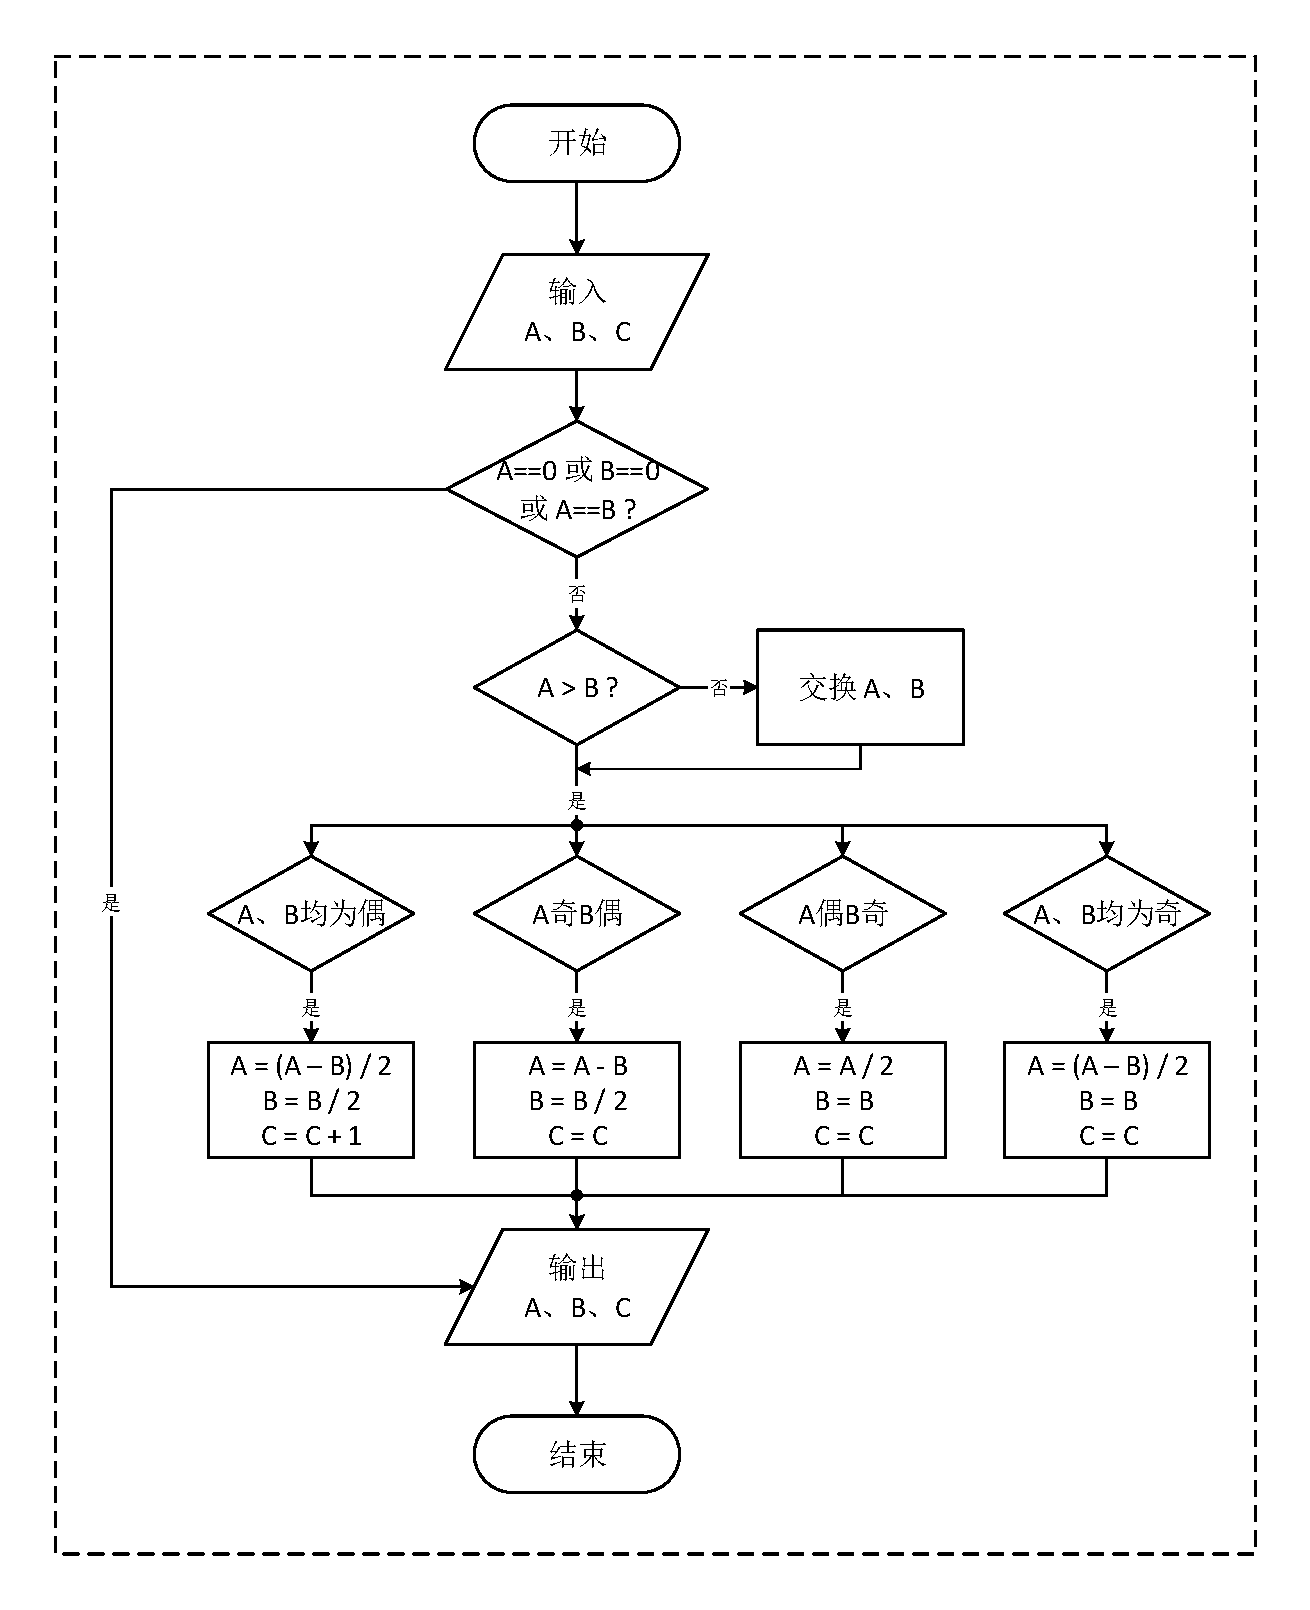
\includegraphics[width=0.9\textwidth]{./yhc_hp/work_flow.eps}
\caption{stein算法流程图}
\end{center}
\end{figure}

原始的stein算法在一次迭代中需要进行比较、减法、移位判断(奇偶判断)、移位四步计算,那么关键路径即包含了32位比较、32位减法、1位比较、移位四部分延时。尽管去除了欧几里得算法中的取余操作,降低了硬件开销和计算延时,但仍然具有改进空间。这里的32位比较和32位减法实际上进行了重复工作,比较是为了保证减法的结果为正,但为了提高性能,我们可以直接将A-B和B-A的减法并行地计算出来,然后使用2路选择器选出为正的结果,得到|A-B|。进一步的,我们发现因为A、B的输出结果只有|A-B|、|A-B|/2、A、A/2、B、B/2这六种情况,我们可以提前将(A-B)/2、(B-A)/2、A/2、B/2并行地计算出来,然后将奇偶判断和上述的正负判断结合为一个更大的8路选择器,得到最终得到A、B输出。改进后的电路图如下图所示。

\begin{figure}[H]
\begin{center}
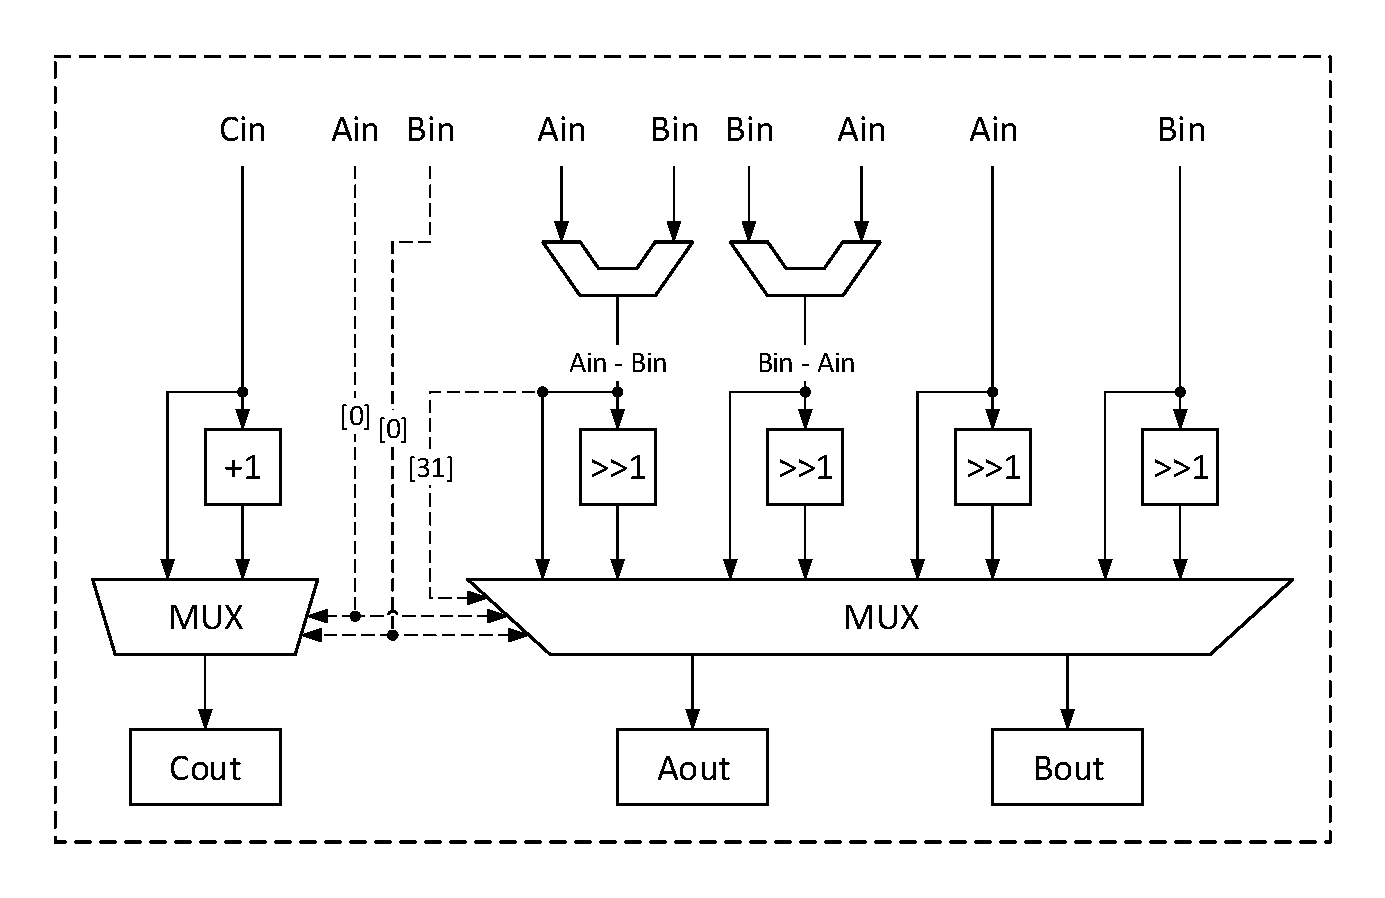
\includegraphics[width=0.8\textwidth]{./yhc_hp/gcd_plc.eps}
\caption{改进后的gcd\_plc模块电路图}
\end{center}
\end{figure}

通过以上的改进,关键路径将仅包含32位减法、移位、多路选择3部分延时,可以去掉延时较高的32位比较操作,大大降低关键路径长度,提高计算性能。

\subsubsection{数据输出模块}
该模块将A、B进行适当的移位并输出,同时给出Done信号。该模块的电路图如下图所示。

\begin{figure}[H]
\begin{center}
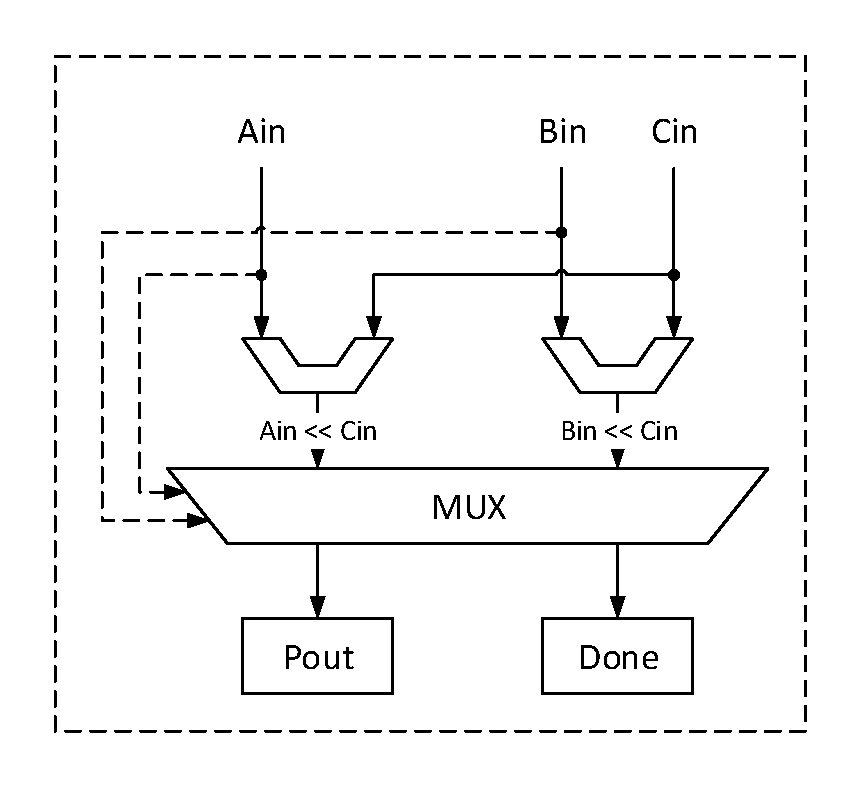
\includegraphics[width=0.5\textwidth]{./yhc_hp/gcd_output.eps}
\caption{gcd\_output模块电路图}
\end{center}
\end{figure}

\subsection{功能验证}
在功能验证中,我们用到了VCS来运行systemverilog的testbench,用dve来观察验证的波形图于debug调试。在功能验证中,我们生成了一万组随机数,并且对比设计时所用的verilog模块得到的结果与c语言模块得到的结果进行对比。其中验证的关键代码如下所示:

\lstset{language=C}
\begin{lstlisting}
for(k = 0; k < 10000; k = k + 1) begin 
	#200;
	if (bus.randomize() == 1);
	else
		$display("Randomization failed");
	opa = bus.NA;
	opb = bus.NB;
	gcdresult = gcd(longint'(bus.NA), longint'(bus.NB));
	#200;
	start = 1'b1;
        #200;
	start = 1'b1;
	#10000000;
	if (desingresult == gcdresult)
		nright = nright + 1;
	else begin 
		$display("operator is: opa = %d , opb = %d", opa, opb);
		$display("two result is not equal: desingresult = %d , gcdresult = %d", desingresult, gcdresult);
		errorFlag = 1'b1;
		nfalse = nfalse + 1;
	end
	if (k % 100 == 0)
		$display("have finish %d percent test", k/100);	
end
\end{lstlisting}

最后验证结果为高性能设计中一万组测试数据全部通过。仿真的systemverilog脚本与仿真结果的log在simulation文件夹中。

\subsection{Vivado综合,功耗、资源占用与时序分析}
我们使用vivado在out of context模式下对高性能设计进行了综合,在xilinx xxx系列芯片上,高性能设计的最高频率可以达到700MHz。700MHz下资源占用情况如下图所示。

\begin{figure}[H]
\begin{center}
\includegraphics[width=0.9\textwidth]{./yhc_hp/700m_utilization.png}
\caption{资源利用}
\label{700m_utilization}
\end{center}
\end{figure}

功耗报告如下图所示。

\begin{figure}[H]
\begin{center}
\includegraphics[width=0.9\textwidth]{./yhc_hp/700m_power.png}
\caption{功耗报告}
\label{700m_power}
\end{center}
\end{figure}

时序报告如下图所示。

\begin{figure}[H]
\begin{center}
\includegraphics[width=0.9\textwidth]{./yhc_hp/700m_timing.png}
\caption{时序报告}
\label{700m_timing}
\end{center}
\end{figure}

通过时序报告可以发现,关键路径存在于gcd\_plc中,和我们在RTL电路设计流水线计算模块一节中的估计相吻合。所以,减法、移位和多路选择构成了电路的关键路径,限制了电路频率的提高。

在100MHz、200MHz、300MHz、400MHz、500MHz、600MHz、700MHz下功耗和资源占用情况(LUT)以及计算得到的能耗比,如下表所示。这里我们以每秒钟可以进行的gcd次数(即吞吐率)作为性能指标,以性能和功耗之比作为能耗比指标。

\begin{table}[H]
\centering
\begin{tabular}{ccccc}
\hline 
& 功耗 W & LUT \%  & 性能 gcd/s & 能耗比 gcd/(sW) \\
\hline 
100 MHZ & 0.959 & 6.20 & 100 & 104.3 \\
200 MHZ & 1.304 & 6.20 & 200 & 153.4 \\
300 MHZ & 1.648 & 6.20 & 300 & 182.0 \\
400 MHZ & 1.993 & 6.21 & 400 & 200.7 \\
500 MHZ & 2.346 & 6.53 & 500 & 217.1 \\
600 MHZ & 2.692 & 6.53 & 600 & 222.9 \\
700 MHz & 3.053 & 6.53 & 700 & 229.3 \\
\hline 
\end{tabular}
\caption{不同频率下的功耗、资源占用和能效比}
\label{hp_power_table}
\end{table}

不同频率下性能和能耗比的曲线如下图所示。
\begin{figure}[H]
\begin{center}
\includegraphics[width=0.7\textwidth]{./yhc_hp/power_table.png}
\caption{不同频率下的功耗和能效比}
\end{center}
\end{figure}

\subsection{基于SoC的验证平台}
\begin{figure}[H]
\begin{center}
\includegraphics[width=0.7\textwidth]{./highperformance/SoCArchitecture.png}
\caption{SoC顶层框图}
\label{SoCArchitecture}
\end{center}
\end{figure}
构建如上图所示的SoC系统,其中gcd模块的访问逻辑较简单,采用由Xilinx公司提供的AXI GPIO作为AXI总线与gcd模块的通信方式。最终实现的硬件框图如下所示。
\begin{figure}[H]
\begin{center}
\includegraphics[width=0.9\textwidth]{./highperformance/SoCSchematic.png}
\caption{SoC电路图}
\label{SoCSchematic}
\end{center}
\end{figure}
其中,System ILA模块用于在调试SoC时,抓取板上信号。

本设计最终运行在时钟频率280Mhz,最终Soc系统的资源占用如下所示。

\begin{figure}[H]
\begin{center}
\includegraphics[width=0.7\textwidth]{./highperformance/Utilization.png}
\caption{资源利用}
\label{Utilization}
\end{center}
\end{figure}
时序报告如下所示。
\begin{figure}[H]
\begin{center}
\includegraphics[width=0.7\textwidth]{./highperformance/Timing.png}
\caption{时序报告}
\label{Timing}
\end{center}
\end{figure}
功耗报告如下所示。
\begin{figure}[H]
\begin{center}
\includegraphics[width=0.7\textwidth]{./highperformance/Power.png}
\caption{功耗报告}
\label{Power}
\end{center}
\end{figure}
将硬件码流烧进FPGA,并将在Xilinx软件开发工具(XSDK)中编写完成的C程序在裸机下运行。C程序如下所示。
\subsubsection{SoC验证代码}
\lstset{language=C}
\begin{lstlisting}[language=c]
#include <stdio.h>
#include "platform.h"
#include "xil_printf.h"
#include <stdlib.h>
#define OPA 	(unsigned int *)0x80000000
#define OPB 	(unsigned int *)0x80010000
#define START 	(unsigned int *)0x80030000
#define DONE 	(unsigned int *)0x80040000
#define RESULT 	(unsigned int *)0x80020000
int gcd_0(int a, int b) {
	if (a%b == 0)
		return b;
	return gcd_0(b, a%b);
}
int gcd(int a, int b) {
	volatile unsigned int *p = OPA; 
	volatile unsigned int *q = OPB; 
	volatile unsigned int *s = START; 
	volatile unsigned int *t = DONE; 
	volatile unsigned int *m = RESULT; 
	*p = a;
	*q = b;
	*s = 1;
	while (*t == 0) {;}
	printf("gcd(%4d,%4d) = %4d,", a, b, *m);
	*s = 0;
	return *m;
}
int main()
{
	init_platform();
	print("*******************\n\r");
	print("start!\n\r");
	print("*******************\n\r");
	int i = 1;
	int a,b;
	while (i <= 20) {
		a = rand() % 10000;
		b = rand() % 10000;
		printf("No.%2d:", i);
		volatile int m = gcd(a, b);
		volatile int k = gcd_0(a, b);
		if (k == m)
			printf("%4d is right!\n\r", k);
		else
			print("ERROR!\n\r");
		i++;
	}
	cleanup_platform();
	return 0;
}
\end{lstlisting}
最终通过UART观察到的结果如下。
\begin{figure}[H]
\begin{center}
\includegraphics[width=0.9\textwidth]{./highperformance/Uart.png}
\caption{UART结果}
\label{Uart}
\end{center}
\end{figure}
测试通过。


\section{低功耗设计}
\subsection{设计综述}
经过第2章中对算法的分析,在低功耗的设计中,我们采用了算法\ref{optimized_stein_algorithm},也就是改进的stein算法。该算法的优势也正如前面分析的一样:
\begin{itemize}
\item 硬件实现简单,只包含\textbf{选择判断有效位数},\textbf{比较},\textbf{移位},\textbf{减法}操作,不含复杂的除法操作。
\item 平均迭代次数为23.7273接近于gcd算法的平均18.2592次迭代
\end{itemize}

所以根据改进的stein算法的优势,我们预期其在低功耗设计中具有很优秀的表现。由于是低功耗设计,我们采用状态机而不是流水线的形式来控制算法流程,这样能够大大减少寄存器的数量和组合逻辑电路的数量,降低电路的静态功耗。而且由于迭代次数短,电路的动态功耗也能被有效降低。

\subsection{状态机设计}
由于采用状态机的设计,根据算法\ref{optimized_stein_algorithm},我们设计了一个状态机,首先定义了状态机的几个状态为:

\begin{description}
\item[IDLE] 表示为空闲状态;
\item[INPUT] 表示为输入采样状态;
\item[ADJUDICATE] 表示判别状态,表示继续输入或者结束运算输出结果
\item[CAMPSWITCH] 表示比较大小,并且交换操作数的位置
\item[ALIGN] 表示使操作数对齐的状态
\item[ABSOLUTE] 表示两操作数相减取绝对值得状态
\item[OUTPUT] 表示输出状态
\end{description}

并且我们定义了状态机的转换框图\ref{statemachine}为:

\begin{figure}[H]
\begin{center}
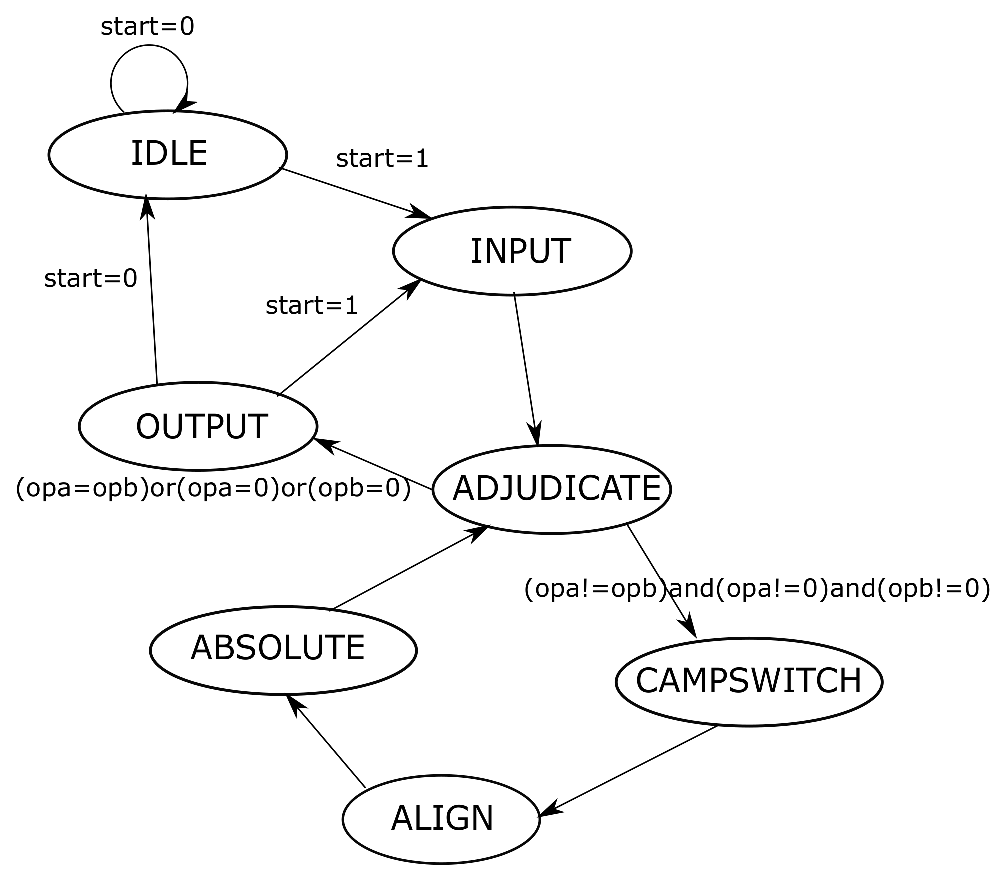
\includegraphics[width=0.6\textwidth]{./lowpowerdesign/low_power_desing_statemachine.eps}
\caption{状态机转换图}
\label{statemachine}
\end{center}
\end{figure}

在改状态机中,首先系统处于IDLE状态,当start信号到来之后,系统开始采样输入,进入INPUT状态。接着从INPUT状态进入ADJUDICATE状态,对两个操作数进行判别,看操作数是否达到可以输出的条件。如果达不到输出的条件,系统计入计算周期$CAMPSWITCH \to ALIGN \to ABSOLUTE \to ADJUDICATE$。计算周期结束之后继续进行判别。如果达到输入条件,系统进入OUTPUT状态并且输出结果。

\subsection{两种低功耗设计}
根据状态机来设计低功耗电路使,我们经过设计迭代,发现有两种低功耗的设计方案,一种是寄存器比较多的设计,一种是组合电路比较多的设计。经过仿真验证与综合分析我们发现两者的功耗相当,寄存器较多的设计比组合电路较多的设计的功耗略大,到时能够达到的最高频率高,关键路径短。经过我们小组讨论分析,绝对这两种方案都适合于做低功耗设计,因此下面来具体说明两种设计方案。为了表示,我们将寄存器较多的设计成为\textbf{register~case},组合电路较多的设计成为\textbf{logic~case}.

\subsection{resgister~case}
首先是resgiste~case——也就是寄存器较多的设计,register~case设计在文件$register_case$中,在这个设计中,我们定义了一系列的寄存器:

\begin{quote}
$current\_state[2:0],next\_state[2:0]
,regopa[31:0],regopb[31:0],
regpa\_out[31:0],
regpb\_out[31:0],tmp\_regopa[31:0],
tmp\_regopb[31:0],
result[31:0],
done,camp\_flag$
\end{quote}

在resgiste~case中一共用掉了232个寄存器。其中$current\_state[2:0],next\_state[2:0]$主要是用于控制状态机的寄存器,$regopa[31:0],regopb[31:0],regpa\_out[31:0],regpb\_out[31:0],tmp\_regopa[31:0],tmp\_regopb[31:0]$是用来暂存操作数的3对寄存器,$result[31:0]$是输出结果的寄存器。$done,camp\_flag$为运算的标志位。下面来对各个模块进行具体的分析。

\subsubsection{比较与交换数据模块}
该模块的主要功能是对暂存在regopa[31:0]和regopb[31:0]上的操作数进行比较大小并且将两者之中较大的数写入寄存器$tmp\_regopa[31:0]$中,将两者中较小的数写入寄存器$tmp\_regopb[31:0]$中,并且根据比较大小的结果写标志位$camp\_flag$。系统接着处理寄存器$tmp\_regopa[31:0]$与寄存器$tmp\_regopb[31:0]$中的数据。该模块的组合逻辑的硬件开销为2个32-bit二路选择器和一个32-bit的比较器。


\begin{figure}[H]
\begin{center}
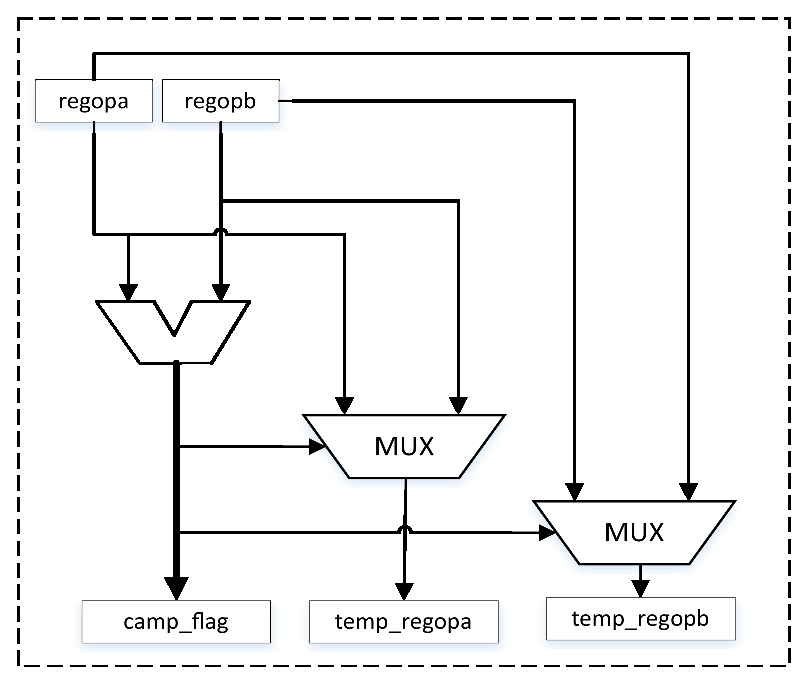
\includegraphics[width=0.7\textwidth]{./lowpowerdesign/camp_switch.eps}
\caption{$CAMP\_SWITCH$模块}
\label{campswitch}
\end{center}
\end{figure}

\subsubsection{对齐模块}
当系统从$CAMP\_SWITCH$状态进入$ALIGN$状态之后,需要根据tmp $\_$ regopa[31:0]与tmp $\_$ regopb[31:0]的数据位宽来进行数据对齐操作。其中在求操作数的有效数据位宽为改设计中最消耗资源的模块。在设计求操作数有效数据位宽的操作中按位判断操作数的有效数据位宽的硬件开销太大而且关键路径很长,因此在设计求操作数有效数据位宽的模块时,我们采用了5层判断,类似于二分法的一个设计,首先判断操作数的高16位是否为0,进而再判断8位、4位、2位、1位,是一种由粗到细判断。这样实现的好处是硬件结构较为对称,电路关键路径短。

\begin{quote}
例如在判断$00000000000000001000000000000000$的有效位位数时,我们先判断高[31:16]为0 $\to$判断[15:8]不为0$\to$判断[15:12]不为0$\to$判断[15:14]不为0$\to$判断[15]不为0,继而得到结果,有效位数为16位。
\end{quote}

求解有效位数的硬件结构框图如下所示:

\begin{figure}[H]
\begin{center}
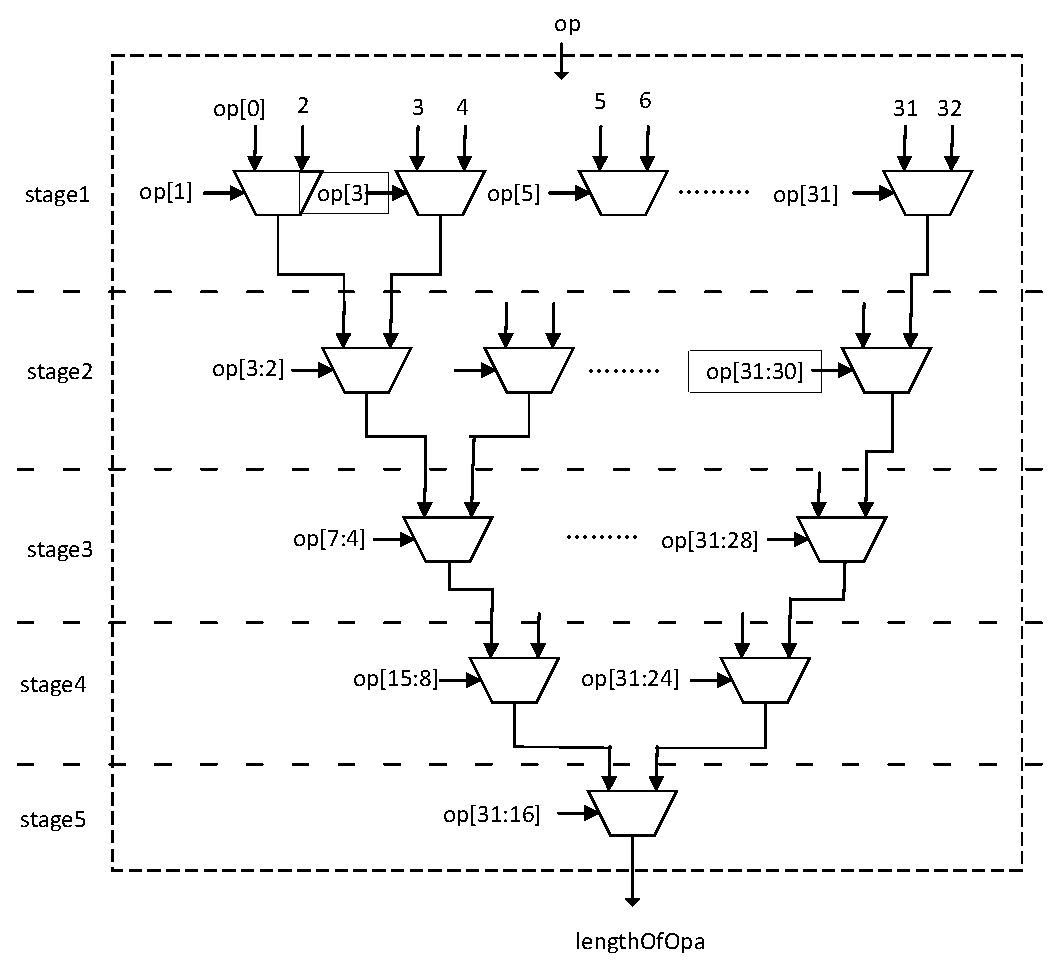
\includegraphics[width=0.7\textwidth]{./lowpowerdesign/length.eps}
\caption{有效位数模块}
\label{length}
\end{center}
\end{figure}

所以有效位数模块中的最长路径为5个二路选择器的延时。

在得到两个操作数的有效位数之后,将两者的有效位数相减便得到有效位数之,差,进而可以对较小的数进行移位操作。所以整个\textbf{对齐模块}的框图如下图\ref{align_model}所示:


\begin{figure}[H]
\begin{center}
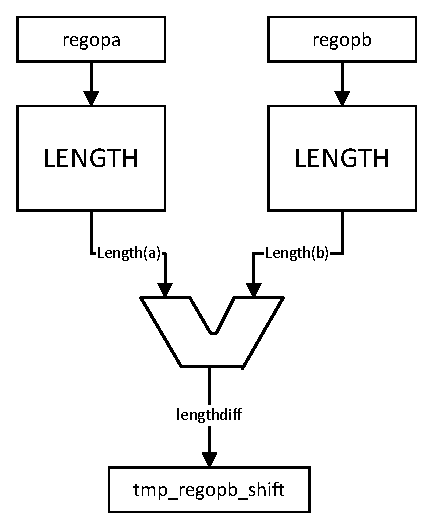
\includegraphics[width=0.5\textwidth]{./lowpowerdesign/align_mdel_logic_case.eps}
\caption{对齐模块}
\label{align_model_logic_case}
\end{center}
\end{figure}

可以看见对齐模块的关键路径长度较长,在关键路径的延时上包括了一个LENGTH模块的延时,一个减法模块的延时,一个移位模块的延时。

\subsubsection{减法求绝对值模块}
在对操作数进行移位之后,进入ABSOLUTE状态,在ABSOLUTE状态中,首先对两个操作数进行大小比较,然后用大数减去小数得到两个操作数的差,用两个操作数的差相减得到结果的绝对值。并且相减得到的绝对值赋值给regopa和regopa和regopb中两个中较小数赋值给regopb(这里需要注意的是,并不是将tmp$\_$regopa和tmp$\_$regopb的较小的数,因为tmp$\_$regopb已经经过移位,将tmp$\_$regopb赋值给regopb会出错),之后再次进入ADJUDICATE,这样一次迭代周期就完成了。

减法求绝对值模块的模块的框图如下所示:

\begin{figure}[H]
\begin{center}
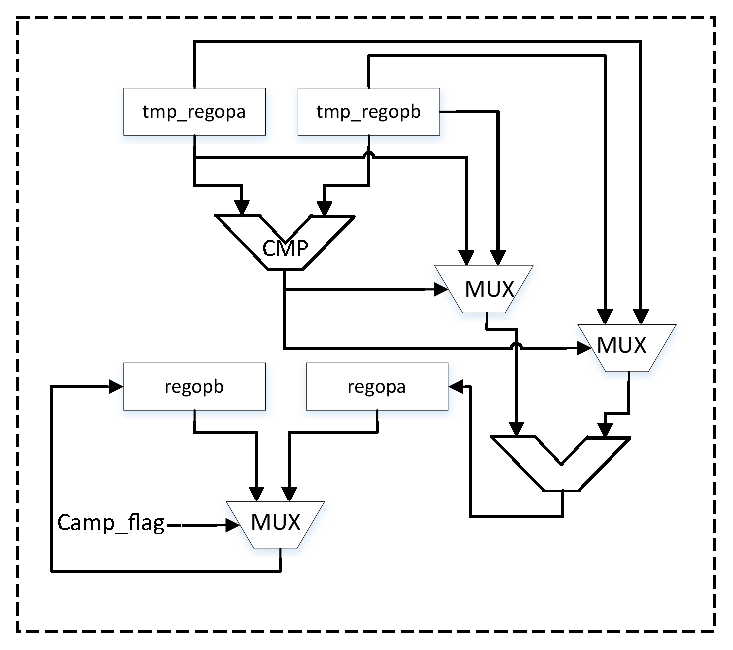
\includegraphics[width=0.7\textwidth]{./lowpowerdesign/abosulate.eps}
\caption{减法求绝对值模块}
\label{align_model}
\end{center}
\end{figure}


\subsection{logic~case设计}
在组合逻辑较多的设计中,我们对寄存器的个数进行了简化,只保留了current$\_$state, next $\_$ state, regopa, regopb, result几个寄存器,将对中间寄存器的操作都合并为对regopa和regopb的操作,并且引入lengt$\_$diff$\_$reg寄存器来暂存两个操作数的有效位数差。这个两个case设计的时候做出的一点改变。因为在logic~case的设计中,只有regopa,regopb两组寄存中,在ALIGN状态之,原始的有效位数信息丢失,所以为了保存原始的有效位数的信息,加入了lengt$\_$diff$\_$reg寄存器来保存历史的有效位数信息。

在logic~case的中只用到了102个寄存器,比原来的resgister~case设计中少了一半以上的寄存器,但是相应的组合逻辑的控制会变复杂,而且由于regopa和regopb在每个状态时刻都会发生改变,在变化时与之相连接的组合逻辑的电路也会发生电路的反转,因而在组合逻辑上会造成更大的功耗,而且由于组合逻辑相应地变得复杂,也会造成关键路径的延时的增加。所以logic~case的设计于resgister~case的设计之间各有利弊。

\subsection{功能验证}
在功能验证中,我们用到了VCS来运行systemverilog的testbench,用dve来观察验证的波形图于debug调试。在功能验证中,我们生成了一万组随机数,并且对比设计时所用的verilog模块得到的结果与c语言模块得到的结果进行对比。其中验证的关键代码如下所示:

\lstset{language=C}
\begin{lstlisting}
for(k = 0; k < 10000; k = k + 1) begin 
	#200;
	if (bus.randomize() == 1);
	else
		$display("Randomization failed");
	opa = bus.NA;
	opb = bus.NB;
	gcdresult = gcd(longint'(bus.NA), longint'(bus.NB));
    #200;
	start = 1'b1;
    #200;
    start=1'b0;
	#1000000;
	if (desingresult == gcdresult);
	else begin 
		$display("operator is: opa=%d, opb=%d", 
		opa, opb);
		$display("two result is not equal:
		desingresult =%d , gcdresult 
		=%d", desingresult, gcdresult);		
		errorFlag = 1'b1;
	end
    if(k % 100==0)
    $display("have finish %d percent test", k/100);		
end
\end{lstlisting}

最后验证结果为logic~case设计中与register~case中一万组测试数据全部通过。仿真的systemverilog脚本与仿真结果的log在simulation文件夹中。

\subsection{DC综合,功耗,面积与时序分析}
在DC综合中我们对于logic~case与register~case设计的不同频率进行综合,发现logic~case的最高频率能够达到500MHZ,register~case设计中的最高频率能够达到600MHZ。因此对logic~case的设计,综合其100MHZ,200MHZ,300MHZ,400MHZ,500MHZ下的不同功耗。对register~case的设计,综合其100MHZ,200MHZ,300MHZ,400MHZ,500MHZ,60
0MZ下的不同功耗。一下是综合得到的结果:


\begin{table}[H]
\centering
\begin{tabular}{ccc}
\hline 
& logic~case & register~case\\
\hline 
100MHZ & 0.1415 mW& 0.2359 mW\\
200MHZ & 0.2840 mW& 0.4773 mW\\
300MHZ & 0.5257 mW& 0.7263 mW\\
400MHZ & 0.6992 mW& 0.9869 mW\\
500MHZ & 1.0016 mW& 1.3718 mW\\
600MHZ &  & 1.8776 mW\\
\hline 
\end{tabular}
\caption{不同频率下的功耗$mw$}
\label{power_table}
\end{table}

\begin{table}[H]
\centering
\begin{tabular}{ccc}
\hline 
& logic~case & register~case\\
\hline 
100MHZ & 4181.039986& 4782.959931\\
200MHZ & 4176.360006& 4913.999997\\
300MHZ & 4807.080038& 4959.360001\\
400MHZ & 5236.560042& 5299.920007\\
500MHZ & 6531.840052& 5937.839956\\
600MHZ &  & 7064.639998\\
\hline 
\end{tabular}
\caption{不同频率下的面积$um*um$}
\label{area_table}

\end{table}

\begin{figure}[H]
\begin{minipage}[t]{0.5\linewidth}
\centering
\includegraphics[width=2.5in]{./powerandarea/power_plot.eps}
\caption{不同频率下的功耗}
\label{power_plot}
\end{minipage}%
\begin{minipage}[t]{0.5\linewidth}
\centering
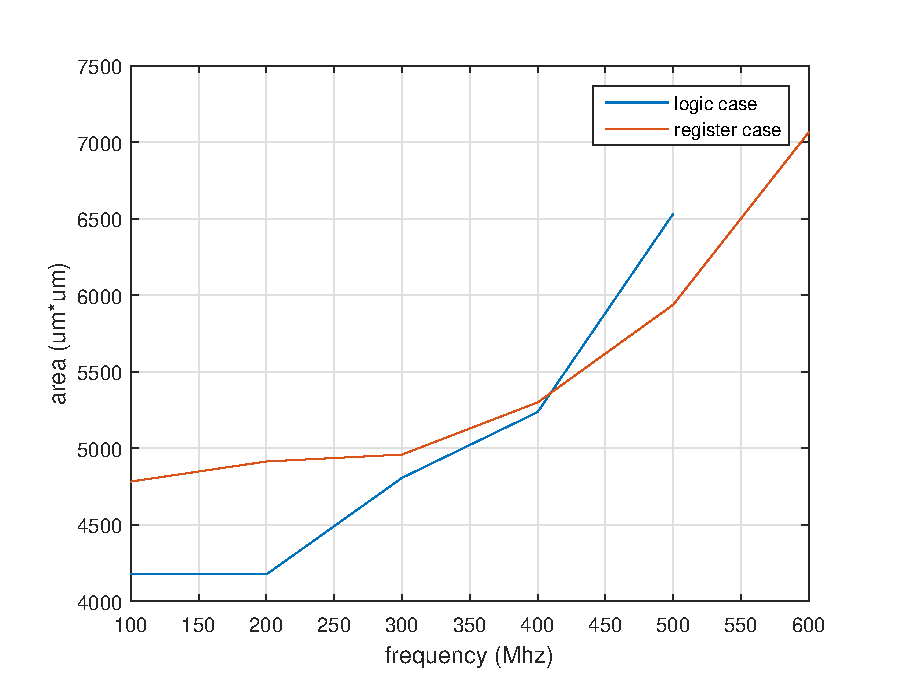
\includegraphics[width=2.5in]{./powerandarea/plot_area.eps}
\caption{不同频率下的面积}
\label{area_plot}
\end{minipage}
\end{figure}


通过观察表\ref{power_table},表\ref{area_table},图\ref{power_plot},\ref{area_plot},可以发现,logic~case因为其寄存器少的原因,功耗比logic~case大,在时序报告中也可以反应出。对于logic~case的设计,寄存器功耗占了约55\%,组合逻辑的功耗占了月45\%。而对于register~case的设计,寄存器的功耗占了约84\%,组合逻辑的功耗占了约16\%。所以在register~case的设计中,寄存器值主要的电路功耗的开销。

在面积报告上,我们也发现一个特点,logic~case的设计面积随着频率增长的速度比较快,而register~case随频率的增长速度比较慢。造成该现象的原因为register~case将组合逻辑切分成比较多的块,每个块在综合的时候相比于logic~case设计中复杂的组合逻辑,综合的不确定性要低。另外一个原因是我们设计中RTL代码使用了比较高层次的行为级语言,而不是更加精确的门级语言,所以综合器有更大的综合空间来优化时序。

对于logic~case的设计,频率的瓶颈在500MHZ,对于register~case的设计,电路时序的瓶颈为600MHZ。通过时序报告得到该设计的关键路径为对其模块中的tmp$\_$regopb的路径,关键路径为下图所示:



\begin{figure}[H]
\begin{minipage}[t]{0.5\linewidth}
\centering
\includegraphics[width=2.5in]{./lowpowerdesign/align_mdel_logic_case_crtical_path.eps}
\caption{logic~case设计关键路径}
\label{gcd_hist}
\end{minipage}%
\begin{minipage}[t]{0.5\linewidth}
\centering
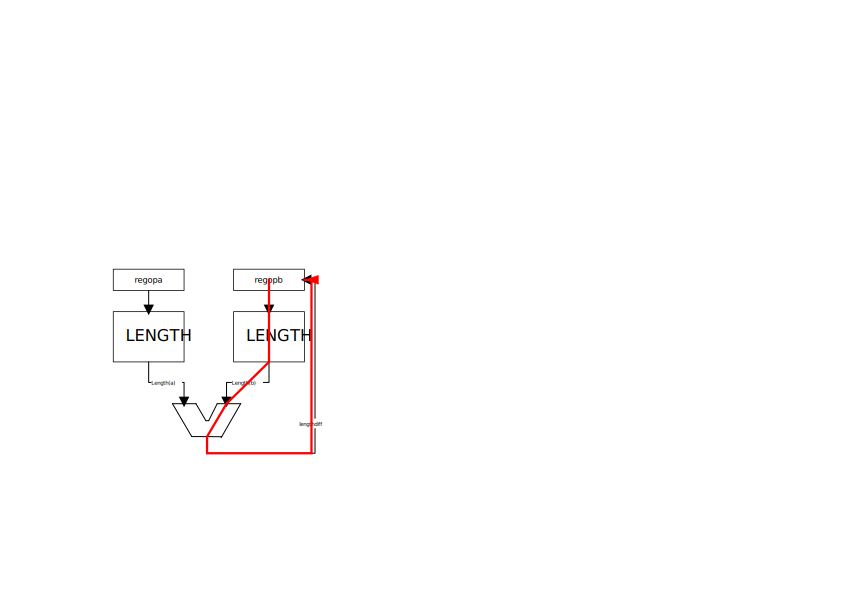
\includegraphics[width=2.5in]{./lowpowerdesign/align_model_register_case_critical_path.eps}
\caption{register~case设计关键路径}
\label{stein_hist}
\end{minipage}
\end{figure}

所以,求操作数的有效位宽,到求解位宽之差,到操作数的移位,这些操作构成了电路的关键路径,限制了电路频率的进一步提高。
\subsection{能效比分析}
电路的能效比为电路处理单位bit数所需要的能量。首先,通过我们仿真得到算法得到结果的平均迭代次数为23.6次,加上输入和输出态各需要占用一个时钟周期,所以总共需要占用约为96.4个周期:
$$1 + 1 + 23.6 \times 4 = 96.4$$
所以能效比计算公式为:
$$efficient = \frac{power \times circle}{frequency \times nBit}$$

经过计算电路的能效比为:

\begin{table}[H]
\centering
\begin{tabular}{ccc}
\hline 
& logic~case & register~case\\
\hline 
100MHZ & 4.2626& 7.1064\\
200MHZ & 4.2777& 7.1893\\
300MHZ & 5.2789& 7.2932\\
400MHZ & 5.2658& 7.4325\\
500MHZ & 6.0346& 8.2651\\
600MHZ &  & 9.4271\\
average & 5.0239 & 7.7856\\
\hline 
\end{tabular}
\caption{不同频率下能效比$fj/bit$}
\label{area_table}

\end{table}

\begin{figure}[H]
\begin{center}
\includegraphics[width=0.7\textwidth]{./powerandarea/efficient.eps}
\caption{不同频率下的能效比}
\label{efficient_model}
\end{center}
\end{figure}

\section{总结}
在这次的课程项目中我们小组首先对求最大公约数的算法进行分析,发现原始的gcd算法进行硬件实现存着很大的开销,不仅电路关键路径长,而且不便于流水线。所以我们小组在对算法进行调研和仿真之后确定了stein算法作为高性能的实现的算法,stein算法硬件实现简单,而且面积开销小,适合于做高性能的流水线实现。在对stein算法做改进之后作为低功耗的实现,改进的stein算法迭代周期短,硬件面积开销小,适合做低功耗的实现。

在高性能的硬件电路实现当中,我们采用了65级流水线,对其关键的gcd\_plc模块进行优化,为了减小电路关键路径,提高电路频率,在gcd\_plc中我们将所有可能的结果并行地计算出来然后通过选择器来选择输出。在FPGA开发板上实现了700MHZ的频率,并且通过了systemverilog仿真随机10000组数据的验证,并且搭建SOC平台进行验证。验证结果表明了电路设计的正确性。

在低功耗的设计中,我们采用了改进的stein算法,设计状态机,并且设计了logic\_case和register\_case,一种组合逻辑比较复杂,另一种寄存器比较多,通过比较发现,logic\_case的功耗比较小,register\_case的频率比较高,而且当综合约束频率上升以后,register\_case所占吗面积比较小。
\section{附录}

\end{document} 